\documentclass[systemskiss/skiss.tex]{subfiles}

\begin{document}

\section{Översikt av projektet}
Projektet kommer vara uppdelat i olika delar. Nedan följer en abstraktion av
hur delarna kan se ut.

\begin{figure}[h]
    \centering
    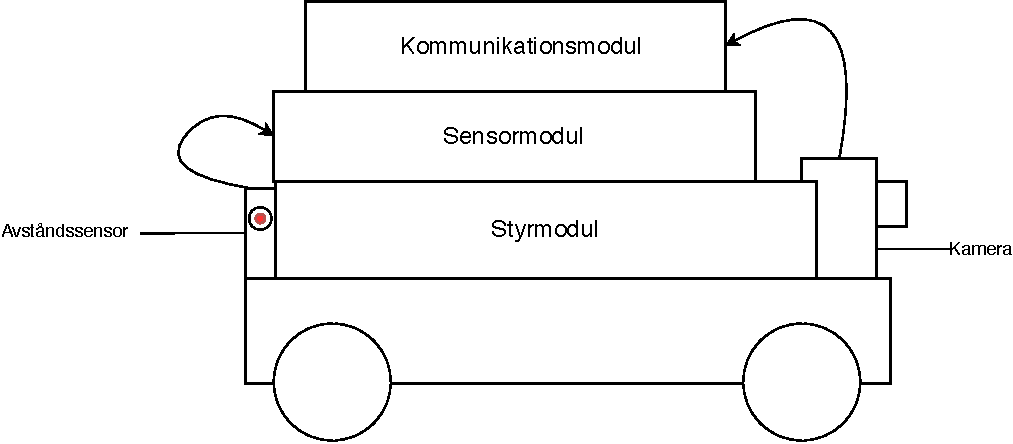
\includegraphics[width=0.6\linewidth]{systemskiss/figures/taxibilen.pdf}
    \caption{Enkel bild av systemets struktur, vardera modul kan vara på
separat virkort. Figuren visar hur virkorten kan staplas på varandra.}
    \label{fig:taxiskiss}
\end{figure}
Figur \ref{fig:taxiskiss} är en bild på hur hela systemet kan se ut när det är
färdigmonterat på chassit. Kameran är riktad framåt för att se vägen bilen kör
på. Sensorer är placerade åt flera olika håll för att mäta avstånd till objekt
i omgivning.

\subsection{Blockschema}

\begin{figure}[h]
    \centering
    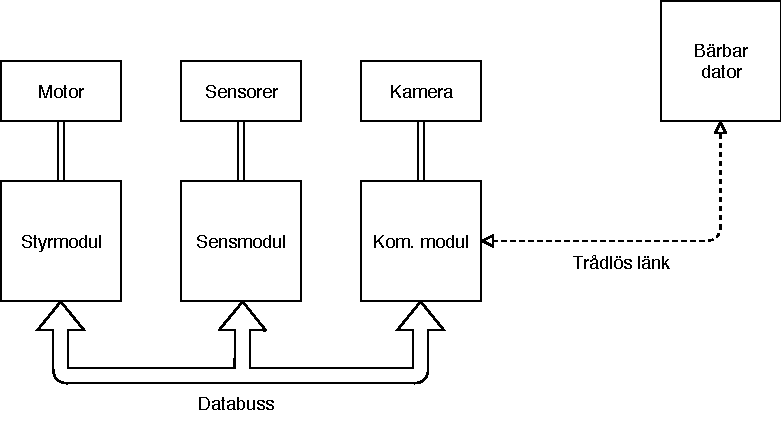
\includegraphics[width=0.6\linewidth]{systemskiss/figures/blockskiss.pdf}
    \caption{Blockschema på systemet}
    \label{fig:blockskiss}
\end{figure}

De tre modulerna är kopplade till en databuss. Bussarna i konstruktionen kommer
antingen vara SPI eller $I_{2}C$. Val av protokoll till databas bestäms under designfasen.
Varje modul är kopplad till den utrustning som respektive modul ansvarar för. Kommunikationsmodulen är även trådlöst kopplad till den bärbara datorn. Figur \ref{fig:blockskiss} visar ett enkelt blockschema för systemets struktur.
 
\subsection{Delsystem och gränssnitt}
Systemet kan främst delas in i moduler, men alla delar kommer inte behöva det. De blir istället delsystem. Kameran är ett delsystem eftersom den inte ingår i någon modul. På samma sätt är den bärbara datorn ett delsystem som trådlöst ska vara kopplad till bilen. 

\subsection{Modularitet och uppgraderbarhet}
Sytemet ska vara moduluppbyggt vilket innebär att man ska kunna byta ut vilken modul som helst mot en annan utan att systemet ska sluta fungera. Efter att systemet är färdigställt ska det också vara lätt att lägga till nya moduler efter behov. Därför ska modulerna kopplas samman med ett bestämt gränssnitt. 

\end{document}

